\section{Systemarchitektur}

\subsection{Grobentwurf}

\begin{figure} 
  \centering
     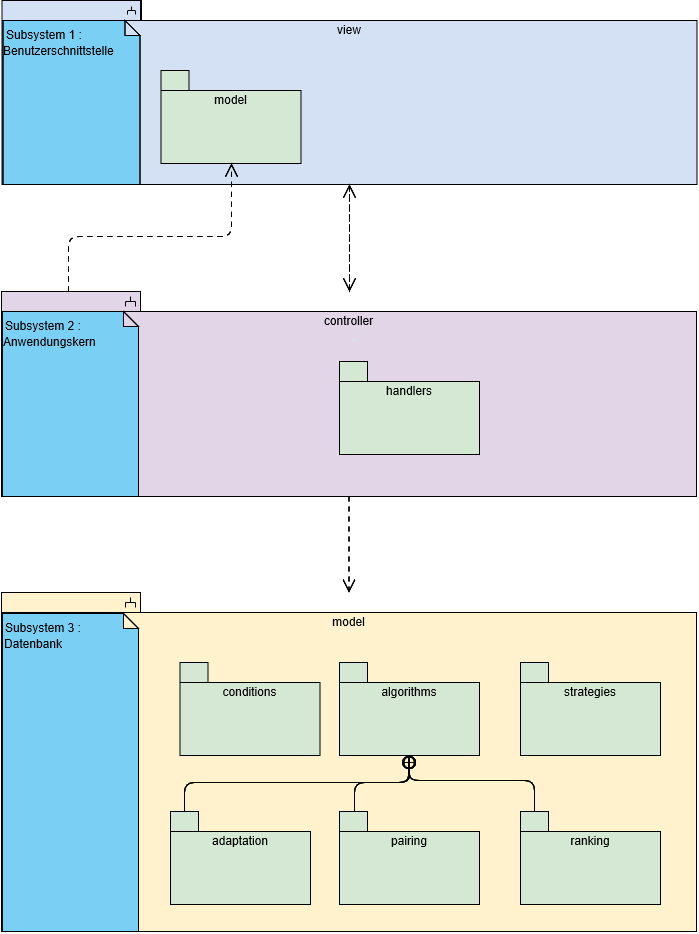
\includegraphics[width=1.1\textwidth]{UMLzuGrobentwurf}
\end{figure}

Sswis baut auf einem MVC-Model auf, welches um ein ViewModel erweitert wurde, was ein vollständiges Abkoppeln von Model und View ermöglicht.
Die Benutzerinteraktion erfolgt über die View. Im ViewModel werden die Benutzereingaben zwischengespeichert und auf Korrektheit überprüft. Des Weiteren schreibt der Controller diejenigen Informationen in das ViewModel, die auf der Benutzeroberfläche angezeigt werden sollen.\\
Der Controller ist für die Programmflusssteuerung zuständig. Die ActionListener der Benutzeroberfläche sind im Controller implementiert. Hierdurch können etwa neue Benutzeroberflächen unter Wiederverwendung der ActionListener erstellt werden.
Außerdem dient der Controller zur Kommunikation zwischen View und Model.\\
Im Model sind die Objekte der Simulation abgebildet. Auch ist hier die gesamte Business Logic implementiert.

\subsection{Controller}

\noindent
\makebox[\textwidth]{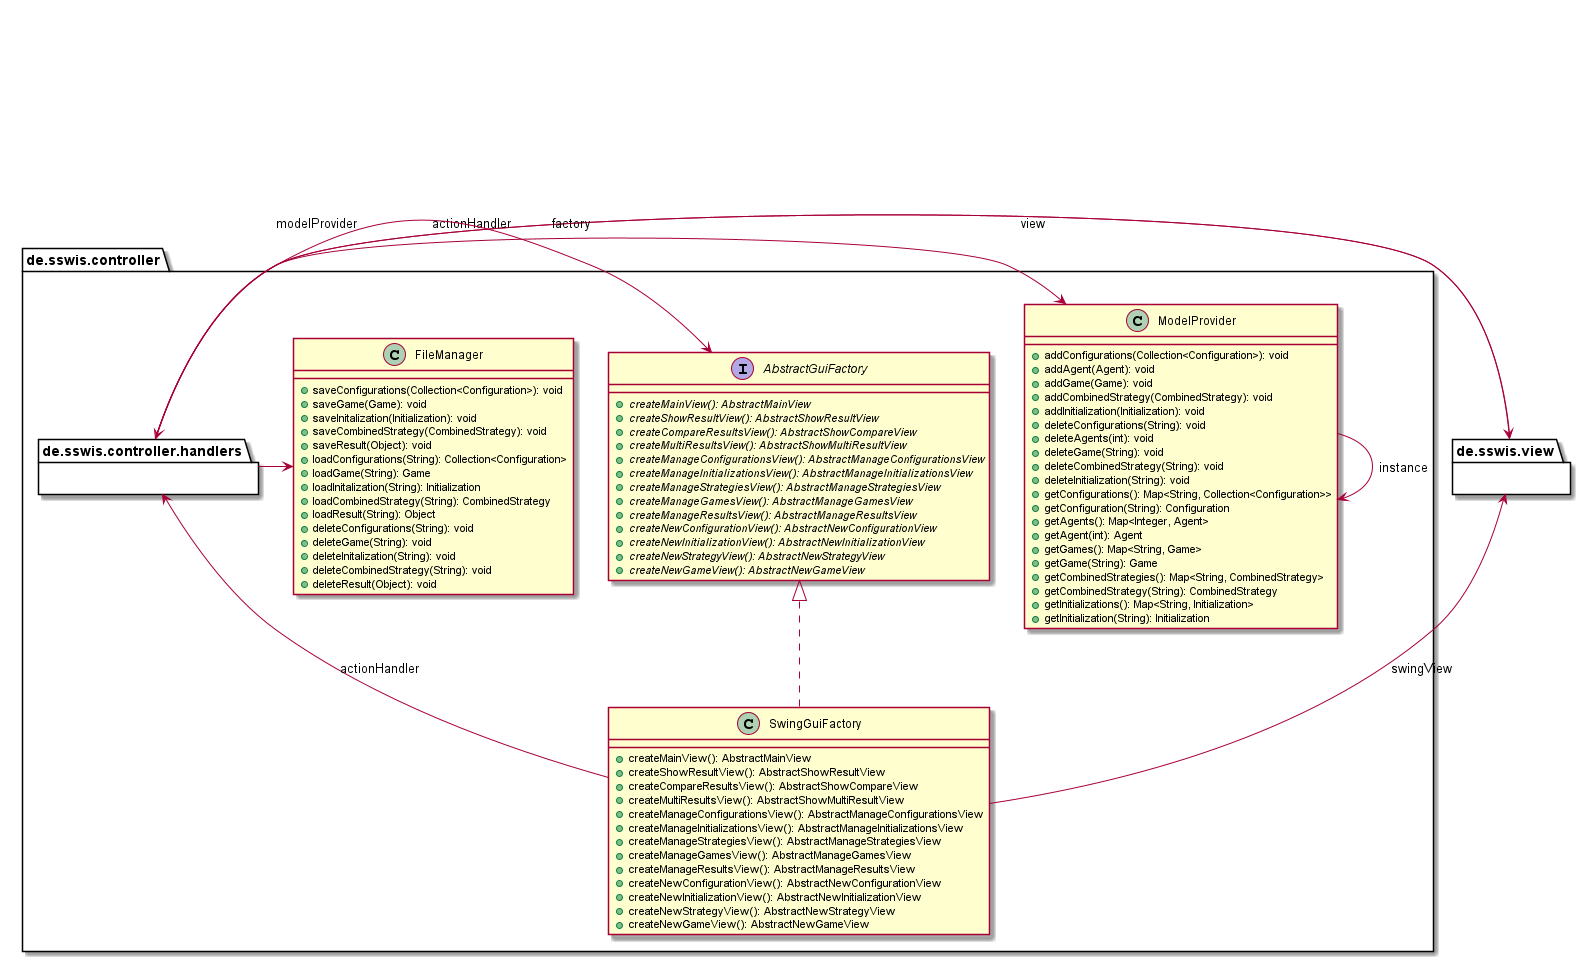
\includegraphics[scale=0.36]{Controller_package}}

Zur Erfüllung der oben angedeuteten Aufgaben steht dem Controller eine Reihe an weiteren Klassen neben den ActionListener-Klassen, die sich im Paket Handlers befinden, zur Verfügung.\\
Zum einen müssen die GUI-Objekte, d.h. alle Fenster mit denen der Benutzer interagiert, erstellt werden. Dies wird durch das Fabrik-Entwurfsmuster realisiert. Das AbstractGuiFactory-Interface gibt alle nötigen Ansichten vor und bietet weiterhin die oben beschriebene Möglichkeit, das Programm zu einem späteren Zeitpunkt komfortabel um neue Benutzeroberflächen zu erweitern.\\
Die SwingGuiFactory-Klasse erstellt die Objekte der von diesem Entwicklerteam angebotenen, Swing-basierten Benutzeroberfläche.

Bei dem ModelProvider handelt es sich um ein Einzelstück, das als zentrale Anlaufstelle für alle Model-Objekte dient. Das Einzelstück-Entwurfsmuster wurde verwendet, um Inkonsistenzen vorzubeugen.

Im FileManager werden Methoden zum Speichern, Laden und Löschen von Objekten bereitgestellt, die gesicherte Benutzereingaben und Ergebnisse darstellen. Das Bearbeiten dieser Objekte geschieht durch ein Laden und anschließendes Speichern des gegebenen Objekts.\\
Die Objekte werden in einem programminternen Verzeichnis gespeichert.

Die vom Programm angebotenen "Dienstleistungen", darunter fallen die diversen Algorithmentypen\footnote{Adaptionsalgorithmen, Paarungsalgorithmen und Bewertungsalgorithmen} sowie die verfügbaren Bedingungen und Basis-Strategien, können durch den ModelServiceLoader zur Verfügung gestellt werden.\\
Dies ist nötig, da sie auf Entwicklerebene um weitere Ausprägungen ergänzt werden können und diese ebenfalls an allen relevanten Stellen, z.B. im Auswahlfenster für den Benutzer, sichtbar sein sollen.

Der ModelParser überträgt das ViewModel in das Model. Konkret werden die im ViewModel auf Korrektheit überprüften Benutzereingaben in Objekte umgewandelt, mit denen eine Simulation durchgeführt werden kann. Andersherum werden die Daten abgelaufener Simulationen in ein Format konvertiert, das die View darstellen kann.

Schließlich können durch das Interface Simulationen überwacht werden, wobei der ViewNotifier die Benutzeroberfläche benachrichtigt, sobald eine Simulation abgeschlossen ist. Es findet eine Parallelisierung statt, wodurch die Benutzeroberfläche auch während einer Simulation aktiv bleibt.

\subsection{Model}

\noindent
\makebox[\textwidth]{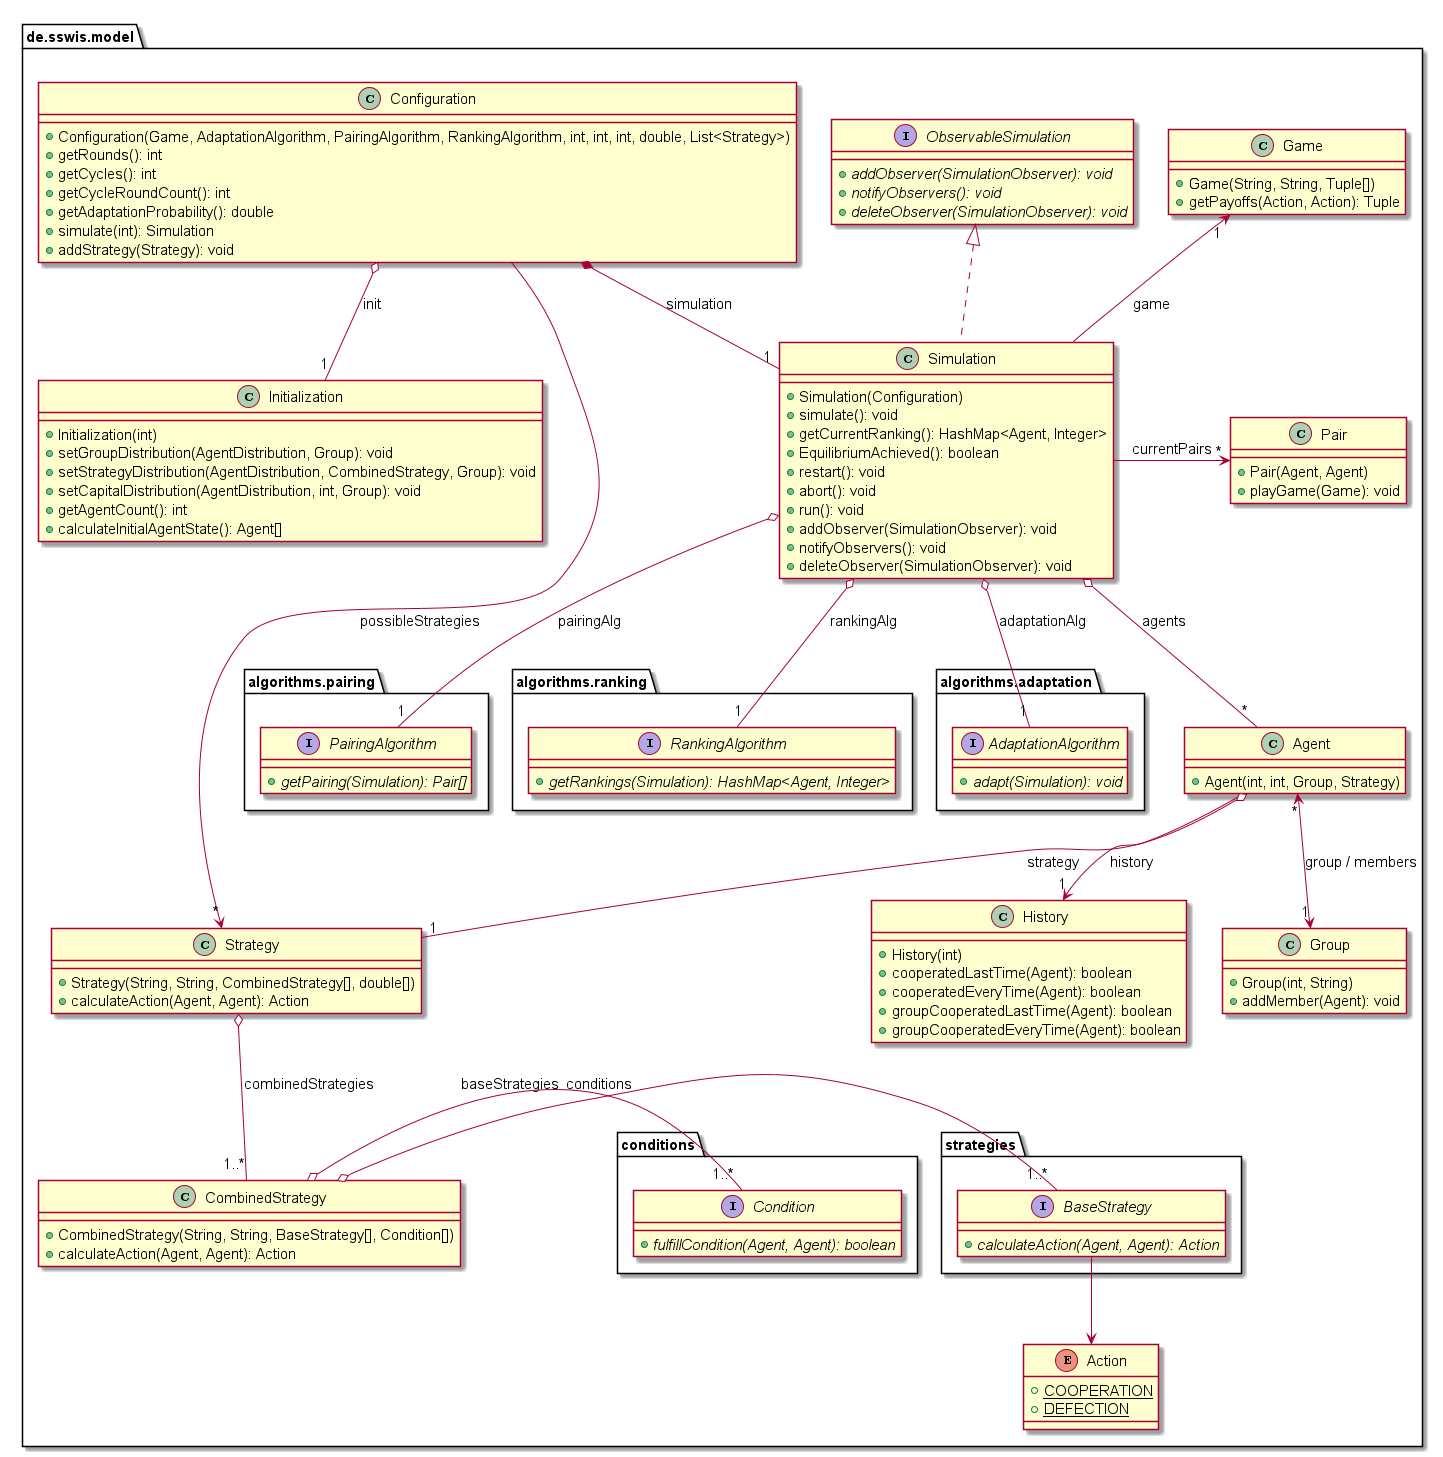
\includegraphics[scale=0.4]{model_classDiagramm}}

Im Model liegen alle Konfigurationen für Erstellen einer Simulation. Für eine Konfiguration gibt es noch eine Initialization, in der die Initiale Konfigurationselemente (zum Beispiel die Art des Spel, die Strategien für die Agenten usw ) zu setzen. \\

Eine Simulation implementiert von einer Schnittstelle OberservableSimulation, um ein Observer zur Simulation hinzuzufügen. Hier wird das Entwurfsmuster Beobachter verwendet. Wenn etwas in Simulation geändert wird, dann sendet der Beobachter der abhängigen Objecten Nachricht.\\

Die Simulation hat die Agenten und in der Simulation werden zwei Agenten durch entsperchendes PairingAlgorithm gepaart, und spielen sie das ausgewälhte Spiel.

Es gibt noch drei Algorithmen Package für die Simulation, das ParingAlgorithm, das RankingAlgorithm und die AdaptionAlgorithm. Das PairingAglorithm bietet die verschiedenen Aglorithmen für die Paarung vom Agenten. Im RankingAlgorithm liegen die Algorithmen für Bewertung. Das AdaptionAlgorithm erhält die Algorithmen, die die Strategien der Agenten in Simulation anpassen. Bei der drei Packages verwendet wir das Entwurfsmuster Strategie, um verschiedene Algorithmen zu bieten.\\

Die Agenten haben die Strategien, und unter den verschiedenen Bedingungen werden die verschiedenen Strategie von Agenten verwendet. Deshalb gibt es hier noch zwei Packages, Condition und BaseStrategy, um die kombinierte Strategien zu erzeugen. Auch wird das Entwurfsmuster Strategie hier bei Condition und BaseStrategy, um verschiedene Bedingungen und einzelstrategien zu bieten. Und hier für Strategie gibt es noch Action "COOPERATION" und "DEFECTION".

Für jeden Agent zeichen wir, dass der Agent zu welcher Gruppe gehört. Und ein History Class wird für Agent erstellt, um einstiges Kooperationsverhalten aufzuzeichen.
